\begin{figure*}[t]
  \centering	
  \begin{subfigure}[t]{.45\linewidth}
    \centering
    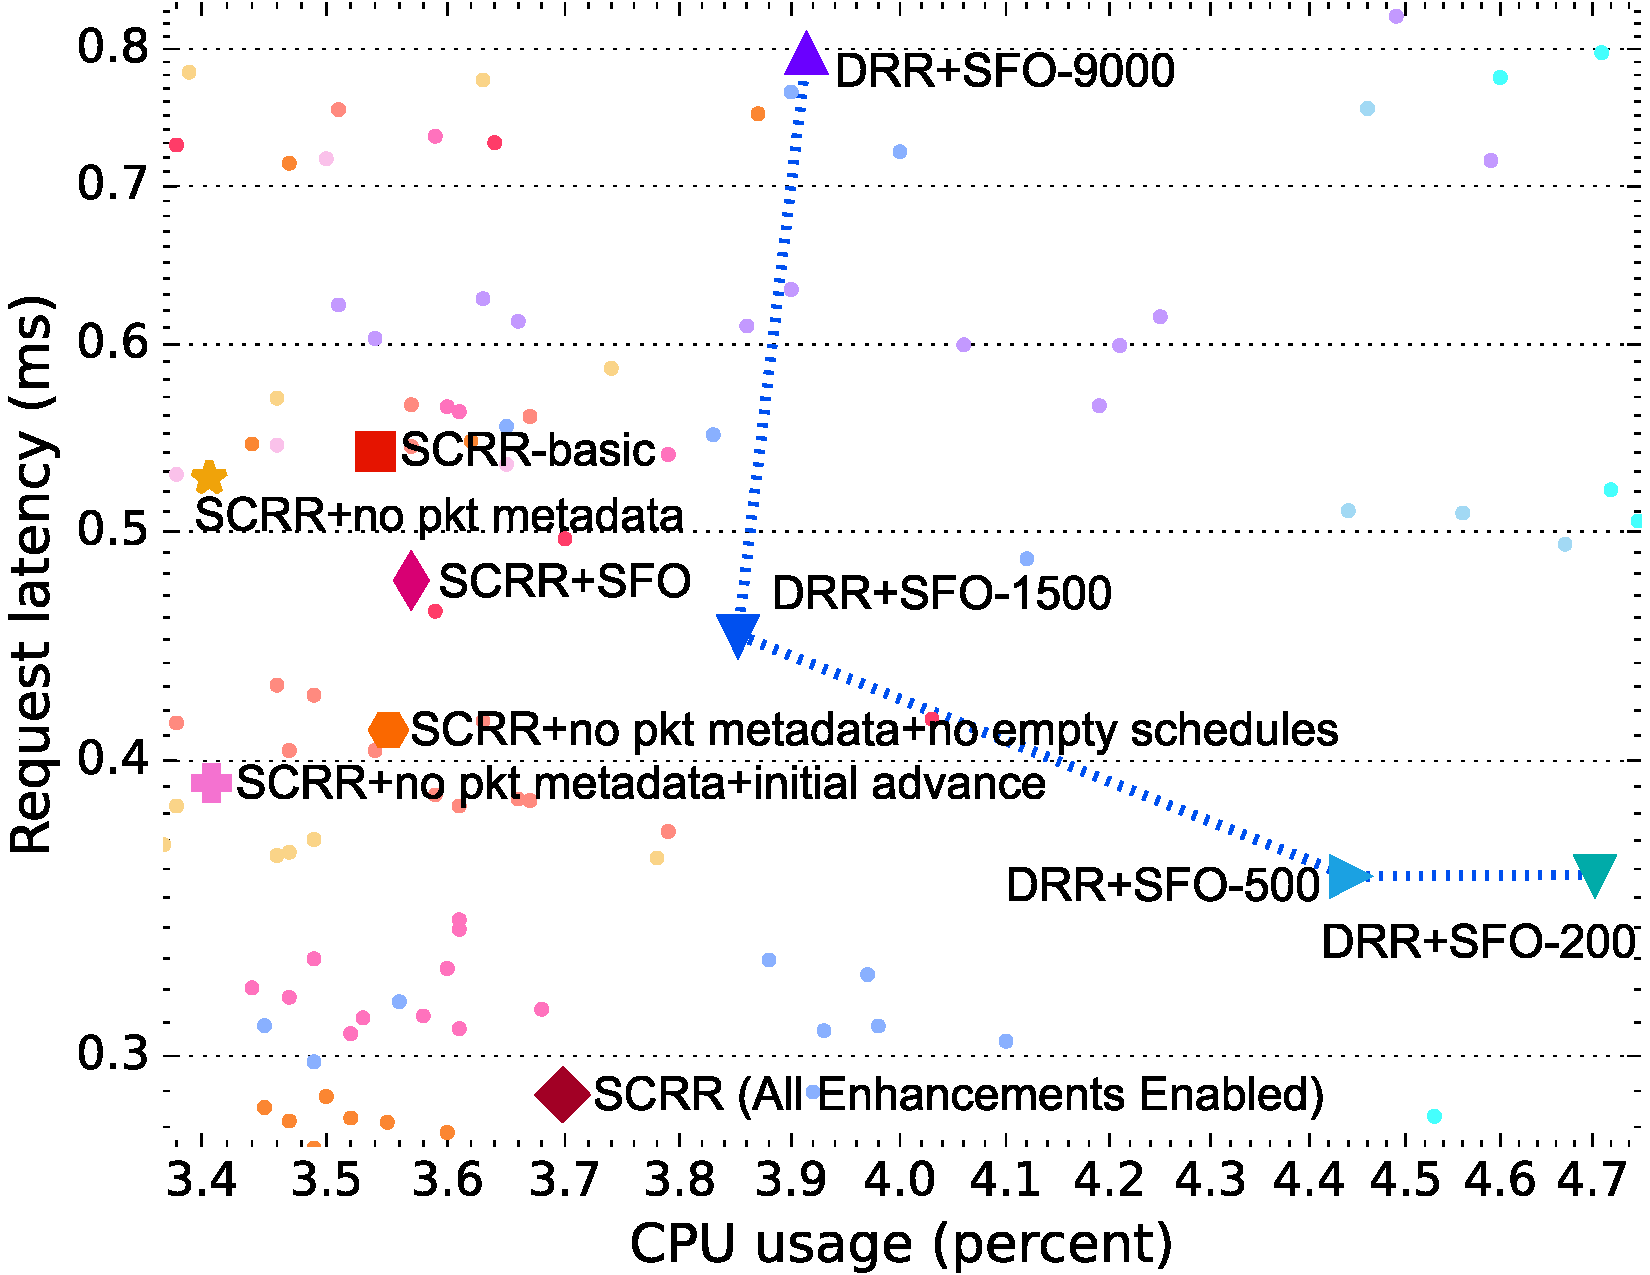
\includegraphics[width=1\linewidth]{figs/component3.pdf}
    % \vspace{-3mm}
    \caption{\small{\textit{CPU utilization vs latency}}}
    \label{fig:component-cpu-lat}
  \end{subfigure}
  \begin{subfigure}[t]{.45\linewidth}
    \centering
    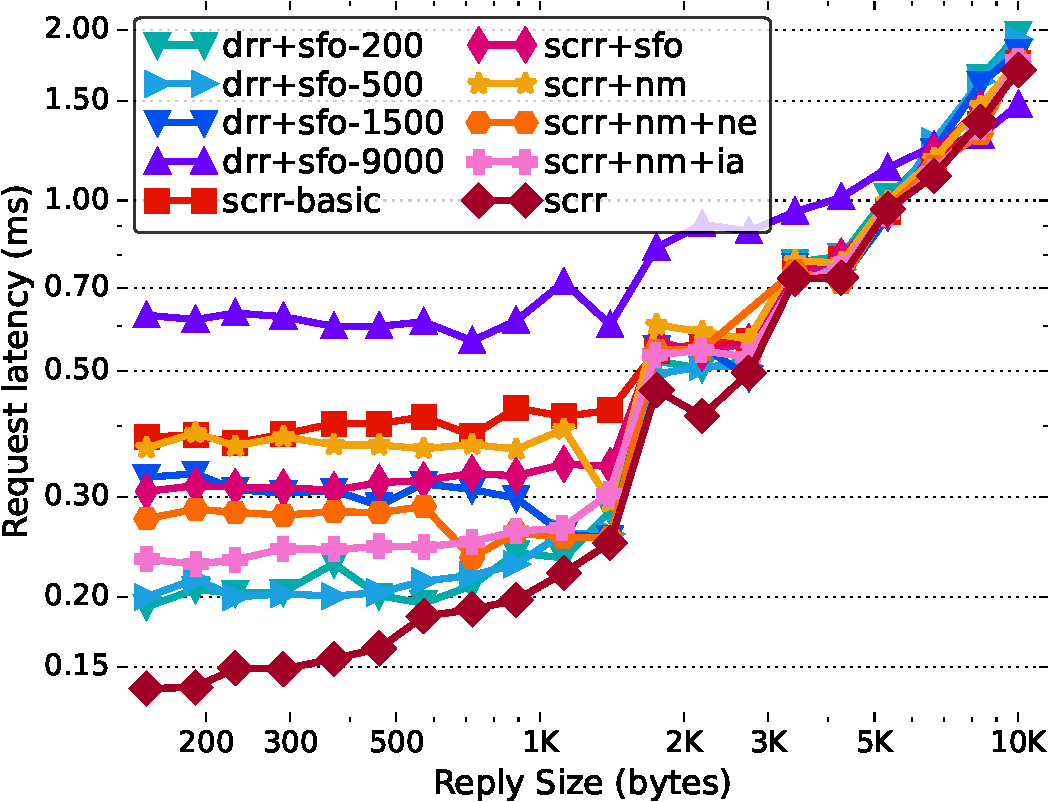
\includegraphics[width=1\linewidth]{figs/component1.pdf}
    % \vspace{-3mm}
    \caption{\small{\textit{Response size vs latency}}}
    \label{fig:component-resp-lat}
  \end{subfigure}
  \begin{subfigure}[t]{.45\linewidth}
    \centering
    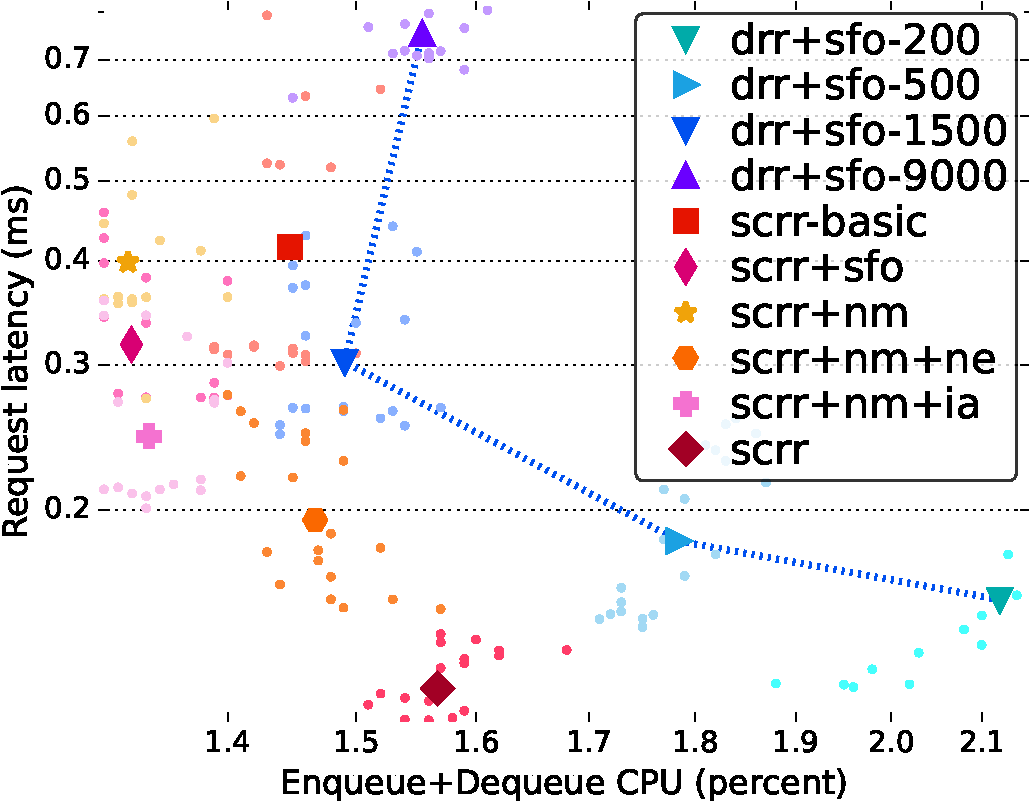
\includegraphics[width=1\linewidth]{figs/pkt_size_edge_cn_2t1x32_mn_2tb1x8_mss_1468_kp_lat_comp_sfonmneia.pdf}
    % \vspace{-3mm}
    \caption{\small{\textit{Edge: Varying Request Size}}}
    \label{fig:component-edge-cpu-lat}
  \end{subfigure}
  \begin{subfigure}[t]{.45\linewidth}
    \centering
    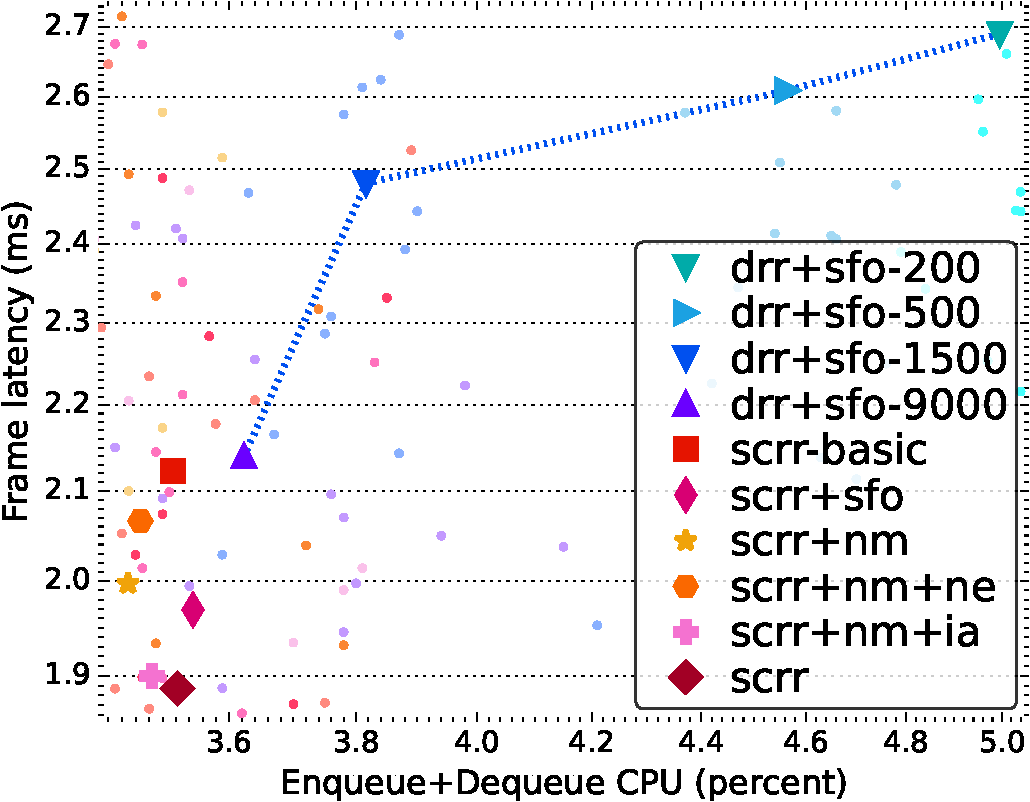
\includegraphics[width=1\linewidth]{figs/pkt_size_cn_2t4x16_mn_2ui32_mss_1468_kp_lat_comp_sfonmneia.pdf}
    % \vspace{-3mm}
    \caption{\small{\textit{Router: Varying VBR pkt size}}}
    \label{fig:component-vbr-cpu-lat}
  \end{subfigure}
  \vspace{-3mm}
  \caption{\small{Comparing the performance of individual SCRR components for the request-response experiment in \S\ref{sec:scrr-eval-latency}.}}
  \label{fig:scrr-component}
  \vspace{-0.2cm}
\end{figure*}
